\section{Connections between Bayesian posterior mean estimators and Hamilton--Jacobi partial differential equations}  \label{sec:connections}

\subsection{Set-up} \label{subsec:set-up}
To establish connections between Bayesian posterior mean estimators and Hamilton--Jacobi equations, we will assume that the regularization term $J$ in the variational imaging model~\eqref{eq:minimization_prob} satisfies the following assumptions:
\begin{enumerate}
    \item[(A1)]  $J\in\gmRn$,
    \item[(A2)]  $\inter(\dom J)\neq \varnothing$,
    \item[(A3)]  $\inf_{\by\in\Rn}J(\by) \in \R$,
and without loss of generality, $\inf_{\by\in\Rn}J(\by)=0$.
\end{enumerate}
Assumption (A1) ensures that the minimal value of the convex imaging problem \eqref{eq:minimization_prob} and its minimizer \eqref{eq:minimizer_prob} are well-defined and enjoy several properties (see Section~\ref{sec:background}, Prop.~\ref{thm:e_u_nonvisc_hj}). Assumption (A2) ensures that for every $\bx \in \Rn$, $t>0$, and $\epsilon > 0$, the posterior distribution
\begin{equation} \label{eq:prob_dist_j}
    \Rn \ni \by \mapsto \frac{e^{-\left(\frac{1}{2t}\left\Vert \bx-\by\right\Vert _{2}^{2}+J(\by)\right)/\epsilon}}{\int_{\Rn}e^{-\left(\frac{1}{2t}\left\Vert \bx-\by\right\Vert _{2}^{2}+J(\by)\right)/\epsilon}\diff\by}
\end{equation}
and its associated partition function
\begin{equation} \label{eq:partition_function}
\Rn\times(0,+\infty)\times(0,+\infty)\ni(\bx,t,\epsilon)\mapsto Z_{J}(\bx,t,\epsilon)=\int_{\Rn}e^{-\left(\frac{1}{2t}\left\Vert \bx-\by\right\Vert _{2}^{2}+J(\by)\right)/\epsilon}\diff\by
\end{equation}
are well-defined, and finally, assumption (A3) guarantees that the partition function~\eqref{eq:partition_function} is also bounded from above independently of $\bx \in \Rn$. We will denote the posterior expectation (with respect to the posterior distribution~\eqref{eq:prob_dist_j}) of a measurable function $f\colon\Omega\mapsto\R$ with $\Omega\subset\dom f$ integrable on the set $\dom f \cap \dom J$ by
\begin{equation} \label{eq:expectation}
\expectationJ{f(\by)}=\frac{1}{Z_J(\bx,t,\epsilon)}\int_{\Omega \, \cap\, \dom J}f(\by)e^{-\left(\frac{1}{2t}\left\Vert \bx-\by\right\Vert _{2}^{2}+J(\by)\right)/\epsilon}\diff\by.
\end{equation}
Posterior expectations of vector quantities are defined similarly component-wise. Posterior expectations generally depends on $(x,t,\epsilon)$ but we will omit writing this dependence explicitly.

\subsection{Connections to viscous Hamilton--Jacobi partial differential equations} \label{subsec:HJ_eqns_visc}
The next proposition establishes connections between viscous HJ PDEs with initial data $J$ satisfying assumptions (A1)-(A3) and both the partition function~\eqref{eq:partition_function} and the Bayesian posterior mean estimate~\eqref{eq:pm_estimate}. These connections mirror those between the first-order HJ PDE~\eqref{eq:hj_non_visc_pde} with initial data $J$ satisfying assumption (A1) and both the convex minimization problem~\eqref{eq:minimization_prob} and the MAP estimate~\eqref{eq:minimizer_prob}. The connections between viscous HJ PDEs and Bayesian posterior mean estimators will be leveraged later to describe several properties of posterior mean estimators in terms of the observed image $\bx$ and parameters $t$ and $\epsilon$, and in particular in Section~\ref{subsec:HJ_eqns_1order} to show that the posterior mean estimate~\eqref{eq:pm_estimate} can be expressed as the minimizer associated to the solution to a first-order HJ PDE (Prop.~\ref{thm:char_opt_sol}) with at least twice continuously differentiable and convex regularization term.

\begin{prop}[The viscous Hamilton--Jacobi equation with initial data in $\gmRn$] \label{thm:visc_hj_eqns} Suppose the function $J$ satisfies assumptions (A1)-(A3). Then the following statements hold.
\begin{enumerate}
\item[(i)] (Cole--Hopf transformation, \cite{evans1998partial} Section 4.4.1) For every $\epsilon>0$, the function $S_\epsilon\colon\Rn\times[0,+\infty)\to[0,+\infty)$ defined by
\begin{equation} \label{eq:hj_s_eps}
S_{\epsilon}(\bx,t)\coloneqq-\epsilon\ln\left(\frac{1}{\left(2\pi t\epsilon\right)^{n/2}}Z_J(\bx,t,\epsilon)\right)=-\epsilon\ln\left(\frac{1}{\left(2\pi t\epsilon\right)^{n/2}}\int_{\Rn}e^{-\left(\frac{1}{2t}\left\Vert \bx-\by\right\Vert _{2}^{2}+J(\by)\right)/\epsilon}\diff\by\right)
\end{equation}
is the unique smooth solution to the viscous HJ PDE with initial data
\begin{equation}
\begin{dcases}\label{eq:hj_visc_pde}
\frac{\partial S_{\epsilon}}{\partial t}(\bx,t)+\frac{1}{2}\left\Vert \nabla_{\bx}S_{\epsilon}(\bx,t)\right\Vert _{2}^{2}=\frac{\epsilon}{2}\Laplacian S_{\epsilon}(\bx,t) & \text{ in }\Rn\times(0,+\infty),\\
S_{\epsilon}(\bx,0)=J(\bx) & \text{ in }\Rn.
\end{dcases}
\end{equation}
In addition, the domain of integration in \eqref{thm:visc_hj_eqns} can be taken to be $\dom J$ or, up to a set of Lebesgue measure zero, $\inter(\dom J)$ or $\dom(\partial J)$. Furthermore, for every $\bx\in\dom J$ and $\epsilon > 0$, except possibly at the boundary points $\bx\in(\dom J)\setminus\inter(\dom J)$ if such points exist, the pointwise limit $S_\epsilon(\bx,t)$ as $t \to 0$ exists and satisfies 
\begin{equation}
    \lim_{\substack{t\to0\\t>0}}S_{\epsilon}(\bx,t)=J(\bx).
\end{equation}
If $\bx\in(\dom J)\setminus\inter(\dom J)$, then we may only conclude 
\[
\liminf_{\substack{t\to0\\t>0}}S_{\epsilon}(\bx,t)\geqslant J(\bx)
\]
 and 
\[\limsup_{\substack{t\to0\\t>0}}S_{\epsilon}(\bx,t)\leqslant J(\bx)-\epsilon\ln\left(\frac{1}{(2\pi\epsilon)^{n/2}}\int_{\dom J}e^{-\frac{1}{2\epsilon}\left\Vert \bx-\by\right\Vert _{2}^{2}}\diff\by\right).
\]

\item[(ii)]  (Convexity and monotonicity properties).
\begin{enumerate}
    \item The function $\Rn\times(0,+\infty)\ni(\bx,t)\mapsto S_{\epsilon}(\bx,t)-\frac{n\epsilon}{2}\ln t$ is jointly convex.
    \item The function $(0,+\infty)\ni t\mapsto S_{\epsilon}(\bx,t)-\frac{n\epsilon}{2}\ln t$ is strictly monotone decreasing.
    \item The function $(0,+\infty)\ni\epsilon\mapsto S_{\epsilon}(\bx,t)-\frac{n\epsilon}{2}\ln\epsilon$ is strictly monotone decreasing.
    \item The function $\Rn \ni \bx \mapsto \frac{1}{2}\normsq{\bx} - tS_\epsilon(\bx,t)$ is strictly convex.
\end{enumerate}

\item[(iii)] (Connections to the posterior mean and mean squared error) The posterior mean estimate $\bu_{PM}(\bx,t,\epsilon)$ and the mean squared error $\expectationJ{\left \Vert \by - \bu_{PM}(\bx,t,\epsilon) \right \Vert_{2}^{2}}$ satisfy the formulas
\begin{equation} \label{eq:grad_s_eps}
    \bu_{PM}(\bx,t,\epsilon) = \bx - t\nabla_{\bx}S_\epsilon(\bx,t)
\end{equation}
and
\begin{equation}\label{eq:exact_variance}
\begin{alignedat}{1}
    \expectationJ{\left \Vert \by - \bu_{PM}(\bx,t,\epsilon) \right \Vert_{2}^{2}} &= t\epsilon \nabla_{\bx}\cdot \bu_{PM}(\bx,t,\epsilon) \\
    &= nt\epsilon - t^2\epsilon\Laplacian S_{\epsilon}(\bx,t).
\end{alignedat}
\end{equation}
Moreover, $\bx \mapsto \bu_{PM}(\bx,t,\epsilon)$ is a bijective function.

\item[(iv)] (Vanishing $\epsilon \to 0$ limit) Let $S_0:\Rn \times (0,+\infty) \to \R$ denote the continuously differentiable and convex solution to the first-order HJ PDE~\eqref{eq:hj_non_visc_pde} with initial data $J$. For every $\bx\in\Rn$ and $t>0$, the following limit holds:
\begin{equation} \label{eq:ldp_limit}
\lim_{\substack{\epsilon\to0\\\epsilon>0}} -\epsilon\ln\left(\frac{1}{\left(2\pi t\epsilon\right)^{n/2}}\int_{\Rn}e^{-\left(\frac{1}{2t}\left\Vert \bx-\by\right\Vert _{2}^{2}+J(\by)\right)/\epsilon}\diff\by\right) = \inf_{\by\in\Rn}\left\{ \frac{1}{2t}\left\Vert \bx-\by\right\Vert _{2}^{2}+J(\by)\right\},
\end{equation}
that is,
\[
\lim_{\substack{\epsilon\to0\\\epsilon>0}}S_{\epsilon}(\bx,t) = S_0(\bx,t),
\]
and the limit converges uniformly over every compact set of $\Rn\times(0,+\infty)$ in $(\bx,t)$. In addition, the gradient $\nabla_{\bx}S_{\epsilon}(\bx,t)$, the partial derivative $\frac{\partial S_{\epsilon}(\bx,t)}{\partial t}$, and the Laplacian $\frac{\epsilon}{2}\Laplacian S_{\epsilon}(\bx,t)$ satisfy the limits
\[
\lim_{\substack{\epsilon\to0\\\epsilon>0}}\nabla_{\bx}S_{\epsilon}(\bx,t)=\nabla_{\bx}S_0(\bx,t), \quad\lim_{\substack{\epsilon\to0\\
\epsilon>0}}\frac{\partial S_{\epsilon}}{\partial t}(\bx,t)=\frac{\partial S_0}{\partial t}(\bx,t),
\]
and
\[
\lim_{\substack{\epsilon\to0\\
\epsilon>0}}\frac{\epsilon}{2}\Laplacian S_{\epsilon}(\bx,t)=0,
\]
where each limit converges uniformly over every compact set of $\Rn\times(0,+\infty)$ in $(\bx,t)$. As a consequence, for every $\bx\in\Rn$ and $t>0$, the pointwise limit of $\bu_{PM}(\bx,t,\epsilon)$ as $\epsilon\to 0$ exists and satisfy
\[
\lim_{\substack{\epsilon\to0\\\epsilon>0}} \bu_{PM}(\bx,t,\epsilon) = \bu_{MAP}(\bx,t),
\]
and the limit converges uniformly over every compact set of $\Rn\times(0,+\infty)$ in $(\bx,t)$.
\end{enumerate}
\end{prop}

\begin{proof}
See Appendix~\ref{app:A}.
\end{proof}

To illustrate certain aspects of Prop.~\ref{thm:visc_hj_eqns} and properties of posterior mean estimates, we give here two analytical examples.

\begin{example}[Tikhonov--Phillips regularization] \label{example:tikhonov}
Let $J(\bx) = \frac{m}{2}\left \Vert \bx \right \Vert_{2}^{2}$ with $m>0$, and consider the solution $S_0(\bx,t)$ and $S_{\epsilon}(\bx,t)$ to the first-order PDE \eqref{eq:hj_non_visc_pde} and viscous HJ PDE \eqref{eq:hj_visc_pde} with initial data $J$, respectively. 

The solution $S_0(\bx,t)$ is given by the Lax--Oleinik formula (Prop.~\ref{thm:e_u_nonvisc_hj}, Eq.~\eqref{eq:lax_formula})
\begin{alignat*}{1}
S_0(\bx,t) & =\inf_{\by\in\Rn}\left\{ \frac{1}{2t}\left\Vert \bx-\by\right\Vert _{2}^{2}+\frac{m}{2}\left\Vert \by\right\Vert _{2}^{2}\right\} \\
& =\frac{m\left\Vert \bx\right\Vert _{2}^{2}}{2(1+mt)}.
\end{alignat*}
This minimization problem is a special case of Tikhonov--Phillips regularization (also known as ridge regression in statistics), a method for regularizing ill-posed problems in inverse problems and statistics using a quadratic regularization term \cite{phillips1962technique,tikhonov1995numerical}. The corresponding minimizer can be computed using the gradient $\nabla_{\bx}S_0(\bx,t)$ via equation \eqref{eq:grad_map_rep} in Prop.~\ref{thm:visc_hj_eqns}:
\begin{equation*}
\bu_{MAP}(\bx,t)  = \bx - t\nabla_{\bx}S_0(\bx,t) = \bx - \frac{mt\bx}{1+mt} = \frac{\bx}{1+mt}.
\end{equation*}

The solution $S_\epsilon(\bx,t)$ is given by the integral
\begin{alignat*}{1}
S_{\epsilon}(\bx,t) & =-\epsilon\ln\left(\frac{1}{(2\pi t\epsilon)^{n/2}}\int_{\Rn}e^{-\left(\frac{1}{2t}\left\Vert \bx-\by\right\Vert _{2}^{2}+\frac{m}{2}\left\Vert \by\right\Vert _{2}^{2}\right)/\epsilon}\diff\by\right)\\
 & =\frac{m\left\Vert \bx\right\Vert ^{2}}{2(1+mt)}+\frac{n\epsilon}{2}\ln\left(1+mt\right).
\end{alignat*}
The posterior mean estimate $\bu_{PM}(\bx,t,\epsilon)$ can be computed using the representation formula~\eqref{eq:grad_s_eps} in Prop.~\ref{thm:visc_hj_eqns}(iii) by calculating the gradient $\nabla_{\bx}S_\epsilon(\bx,t)$:
\begin{equation*}
\bu_{PM}(\bx,t,\epsilon)  = \bx - t\nabla_{\bx}S_\epsilon(\bx,t) = \bx - \frac{mt\bx}{1+mt} = \frac{\bx}{1+mt}.
\end{equation*}
The mean squared error $\expectationJ{\normsq{\by-\bu_{PM}(\bx,t,\epsilon)}}$ can be computed using the representation formula~\eqref{eq:exact_variance} in Prop.~\ref{thm:visc_hj_eqns}(iii) by calculating the divergence of $\bu_{PM}(\bx,t,\epsilon)$:
\begin{equation}\label{eq:tikhonov_var}
    \expectationJ{\left \Vert \by - \bu_{PM}(\bx,t,\epsilon)\right \Vert_{2}^{2}} = t\epsilon \nabla_{\bx} \cdot \bu_{PM}(\bx,t,\epsilon) = \frac{nt\epsilon}{1+mt}.
\end{equation}

Comparing the solutions $S_0(\bx,t)$ and $S_\epsilon(\bx,t)$, we see that $\lim_{\substack{\epsilon\to0\\
\epsilon>0}}S_{\epsilon}(\bx,t)=S_0(\bx,t)$ for every $\bx\in\Rn$ and $t>0$, in accordance to the result established in Prop.~\ref{thm:visc_hj_eqns}(iv). Note also that while $(\bx,t)\mapsto S_0(\bx,t)$ is jointly convex, its viscous counterpart $(\bx,t)\mapsto S_\epsilon(\bx,t)$ is not. Indeed, $t \mapsto S_\epsilon(\bx,t)$ is not convex, and it is convex only after subtracting $\frac{n\epsilon}{2}\ln t$ from $S_{\epsilon}(\bx,t)$.
\end{example}

\begin{example}[Soft thresholding] \label{ex:smooth_shrink} 
Let $J(\bx)=\sum_{i=1}^{n}\lambda_{i}\left|\bx_{i}\right|$, where $\lambda_{i}>0$ for each $i\in\{1,\dots,n\}$, and consider the solutions $S_0(\bx,t)$ and $S_{\epsilon}(\bx,t)$ to the first-order \eqref{eq:hj_non_visc_pde} and viscous HJ PDEs \eqref{eq:hj_visc_pde} with initial data $J$, respectively.

The solution $S_0(\bx,t)$ is given by the Lax--Oleinik formula
\begin{align*}
S_{0}(\bx,t) & =\inf_{\by\in\Rn}\left\{ \frac{1}{2t}\left\Vert \bx-\by\right\Vert _{2}^{2}+\sum_{i=1}^{n}\lambda_{i}\left|y_{i}\right|\right\} \label{eq:ex_sol_eps_0}\\
 & =\sum_{i=1}^{n}\left(\inf_{y_{i}\in\R}\left\{ \frac{1}{2t}(x_{i}-y_{i})^{2}+\lambda_{i}\left|y_{i}\right|\right\} \right),
\end{align*}
where $x_i$ and $y_i$ denote the $i^{\rm th}$ component of the vectors $\bx$ and $\by$, respectively. In the context of imaging, this minimization problem corresponds to denoising an image with the weighted sum of a quadratic fidelity term and a weighted $l_{1}$-norm as the regularization term. This term is widely used in imaging to encourage sparsity of an image, and it has received considerable interest due to its connection with compressed sensing reconstruction \citep{candes2006robust,donoho2006compressed}. The solution to this minimization problem corresponds to a soft thresholding applied component-wise to the vector $\bx$ \cite{daubechies2004iterative, figueiredo2001wavelet,lions1979splitting}. The soft thresholding operator is defined for any real number $a$ and positive real number $\alpha$ as
\begin{equation} \label{eq:thresholding_operator}
\R \times (0,+\infty) \ni (a,\alpha) \mapsto T(a,\alpha)=\begin{cases}
a-\alpha & \mbox{if }a>\alpha,\\
0 & \mbox{if }a\in[-\alpha,\alpha],\\
a+\alpha & \mbox{if }a<-\alpha.
\end{cases}
\end{equation}
The minimizer in the Lax--Oleinik formula of $S_0(\bx,t)$ is then given component-wise for $i\in\{1,\dots,n\}$ by
\[
\left(\bu_{MAP}(\bx,t)\right)_{i}=T(x_{i},t\lambda_{i}),
\]
so that
\begin{equation*}
S_{0}(\bx,t) = \sum_{i=1}^{n}\left( \frac{1}{2t}(x_{i}-T(x_{i},t\lambda_{i}))^{2}+\lambda_{i}\left|T(x_{i},t\lambda_{i})\right|\right).
\end{equation*}

The solution $S_\epsilon(\bx,t)$ is given by the integral
\begin{align*}
S_{\epsilon}(\bx,t) & =-\epsilon\ln\left(\frac{1}{(2\pi t\epsilon)^{n/2}}\int_{\Rn}e^{-\left(\frac{1}{2t}\left\Vert \bx-\by\right\Vert _{2}^{2}+\sum_{k=1}^{n}\lambda_{i}\left|y_{i}\right|\right)/\epsilon}\diff\by\right)\\
 & =-\epsilon\sum_{i=1}^{n}\ln\left(\frac{1}{2}\sqrt{\frac{2}{\pi t\epsilon}}\int_{-\infty}^{+\infty}e^{-\left(\frac{1}{2t}(x_{i}-y_i)^{2}+\lambda_{i}\left|y_i\right|\right)/\epsilon}\diff y_i\right)\\
 & =-\epsilon\sum_{i=1}^{n}\ln\left(\frac{1}{2}\sqrt{\frac{2}{\pi t\epsilon}}\left(\int_{0}^{+\infty}e^{-\left(\frac{1}{2t}(x_{i}+y_i)^{2}+\lambda_{i}y_i\right)/\epsilon}\diff y_i + \int_{0}^{+\infty}e^{-\left(\frac{1}{2t}(x_{i}-y_i)^{2}+\lambda_{i}y_i\right)/\epsilon}\diff y_i\right)\right)
\end{align*}
To compute this integral, first define the function
\begin{equation*}
    \R \ni z \mapsto L(z) = \frac{1}{2}e^{z^2}\erfc\left(z\right),
\end{equation*}
where $\erfc$ denotes the complementary error function. Then we have (\citep{gradshte2007table}, page 336, integral 3.332, 2., and page 887, integral 8.250, 1.)
\begin{equation*}
    \frac{1}{2}\sqrt{\frac{2}{\pi t\epsilon}}\int_{0}^{+\infty}e^{-\left(\frac{1}{2t}(x_{i}+y_i)^{2}+\lambda_{i}y_i\right)/\epsilon}\diff y_i = e^{-\frac{x_{i}^2}{2t\epsilon}}L\left(\frac{x_i + t\lambda_i}{\sqrt{2t\epsilon}}\right)
\end{equation*}
and
\begin{equation*}
    \frac{1}{2}\sqrt{\frac{2}{\pi t\epsilon}}\int_{0}^{+\infty}e^{-\left(\frac{1}{2t}(x_{i}-y_i)^{2}+\lambda_{i}y_i\right)/\epsilon}\diff y_i = e^{-\frac{x_{i}^2}{2t\epsilon}}L\left(\frac{-x_i + t\lambda_i}{\sqrt{2t\epsilon}}\right),
\end{equation*}
from which we get
\begin{equation*}
S_{\epsilon}(\bx,t)=\frac{\left\Vert \bx\right\Vert _{2}^{2}}{2t} -\epsilon\sum_{i=1}^{n}\ln\left(L\left(\frac{x_i + t\lambda_i}{\sqrt{2t\epsilon}}\right) + L\left(\frac{-x_i + t\lambda_i}{\sqrt{2t\epsilon}}\right)\right).
\end{equation*}
Now, to compute the posterior mean estimate it suffices to compute the gradient of $\nabla_{\bx}S_\epsilon(\bx,t)$ and use the formula $\bu_{PM}(\bx,t,\epsilon) = \bx - t\nabla_{\bx}S_\epsilon(\bx,t)$. To do so, we must compute the derivative of the function $L$. Since 
\begin{equation*}
    \frac{dL}{dz}(z) = 2zL(z)+\frac{1}{\sqrt{\pi}},
\end{equation*}
the chain rule gives 
\begin{equation*}
    \frac{\partial}{\partial x_i}\left(L\left(\frac{x_i + t\lambda_i}{\sqrt{2t\epsilon}}\right) + L\left(\frac{-x_i + t\lambda_i}{\sqrt{2t\epsilon}}\right)\right)  = \left(\frac{x_i + t\lambda_i}{t\epsilon}\right)L\left(\frac{x_i + t\lambda_i}{\sqrt{2t\epsilon}}\right) - \left(\frac{-x_i + t\lambda_i}{t\epsilon}\right)L\left(\frac{-x_i + t\lambda_i}{\sqrt{2t\epsilon}}\right).
\end{equation*}
The posterior mean estimate is therefore given component-wise by
\begin{alignat*}{1}
    (\bu_{PM}(\bx,t,\epsilon))_{i} & = x_i - t(\nabla_{\bx}S_\epsilon(\bx,t))_i\\
    & = x_i + t\lambda_i\left(\frac{L\left(\frac{x_i + t\lambda_i}{\sqrt{2t\epsilon}}\right) + L\left(\frac{-x_i + t\lambda_i}{\sqrt{2t\epsilon}}\right)}{L\left(\frac{x_i + t\lambda_i}{\sqrt{2t\epsilon}}\right) - L\left(\frac{-x_i + t\lambda_i}{\sqrt{2t\epsilon}}\right)}\right)
\end{alignat*}

The posterior mean estimate $\bu_{PM}(\bx,t,\epsilon)$ yields a smooth analogue of the soft thresholding operator $T$ (defined in \eqref{eq:thresholding_operator}) evaluated at $(x_i,t\lambda_i)$, in the sense that $\lim_{\substack{\epsilon\to0\\\epsilon>0}} (\bu_{PM}(\bx,t,\epsilon))_i = T(x_{i},t\lambda_{i})$ for every $i\in\{1,\dots,n\}$ by Prop.~\ref{thm:visc_hj_eqns}(iv). Figure~\ref{fig:sparsity_example} shows the MAP and posterior mean estimates in one dimension for the choice of $t=1.25$, $\epsilon=\left\{ 0.025,\,0.1,\,0.25,\,0.5,\,1\right\} $, and $\lambda_{1}=2$ for $x\in[-5,5]$.
\begin{figure}[h]
\centering
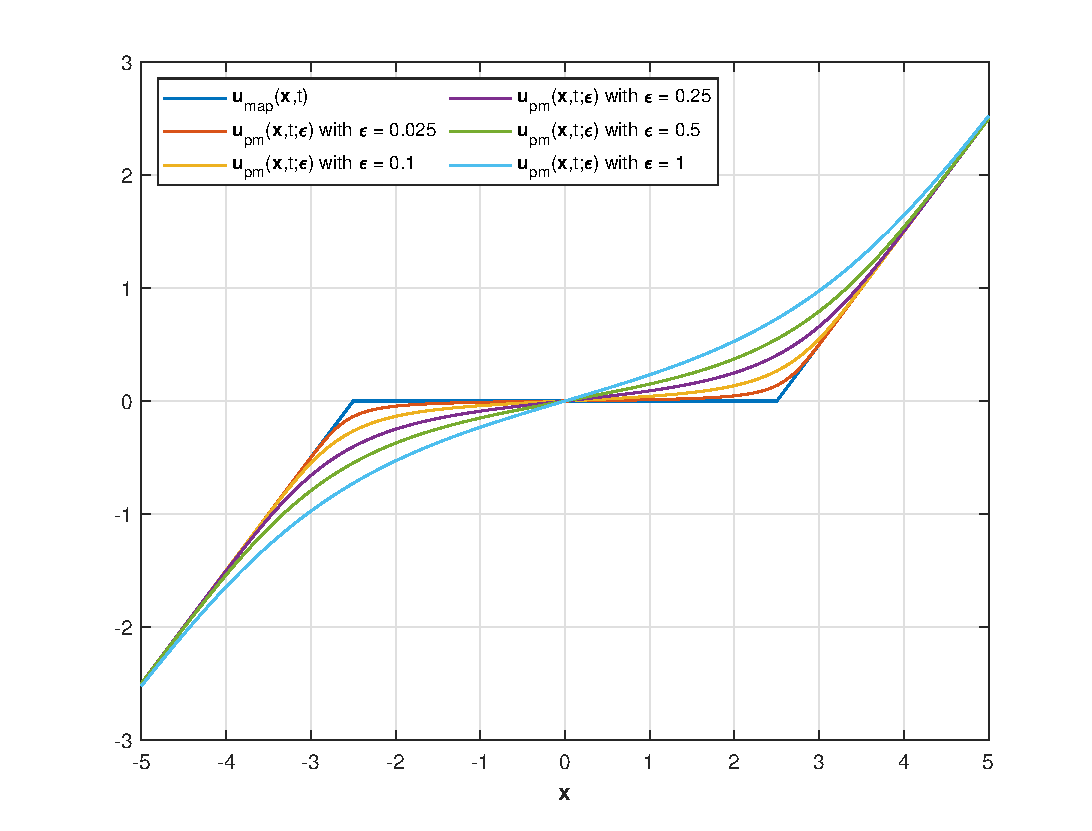
\includegraphics[width=0.75\textwidth]{u_pm_example_figure.pdf}
\caption{Numerical example of the MAP and posterior mean estimates in one dimension with $J(x)=\lambda_{1}\left|x\right|$ for the choice of $t=1.25$, $\epsilon=\left\{ 0.025,\,0.1,\,0.25,\,0.5,\,1\right\}$, and $\lambda_{1}=2$ for $x\in[-5,5]$.}
\label{fig:sparsity_example}
\end{figure}
\end{example}

\subsection{Connections to first-order Hamilton--Jacobi equations} \label{subsec:HJ_eqns_1order}

In this section, we use the connections between the posterior mean estimate~\eqref{eq:pm_estimate} and viscous HJ PDEs established in Prop.~\ref{thm:visc_hj_eqns} to show that the posterior mean estimate can be expressed through the solution to a first-order HJ PDE with initial data of the form of~\eqref{eq:hj_non_visc_pde}. In particular, we show that the posterior mean estimate satisfies the proximal mapping formula
\begin{equation*}
\bu_{PM}(\bx,t,\epsilon) = \argmin_{\by\in\Rn}\left\{ \frac{1}{2}\left\Vert \bx-\by\right\Vert _{2}^{2} + \left(K^{*}_{\epsilon}(\by,t)-\frac{1}{2}\Vert \by \Vert_{2}^{2}\right)\right\},
\end{equation*}
where the function $K_\epsilon\colon\Rn\times\times(0,+\infty) \to \R$ is defined through the solution $S_\epsilon(\bx,t)$ to the viscous HJ PDE~\eqref{eq:hj_visc_pde} via
\begin{equation*}
K_{\epsilon}(\bx,t) \coloneqq \frac{1}{2}\left\Vert \bx\right\Vert _{2}^{2}-tS_{\epsilon}(\bx,t) \equiv t\epsilon\ln\left(\frac{1}{(2\pi t\epsilon)^{n/2}}\int_{\dom J}e^{\left(\frac{1}{t}\left\langle \bx,\by\right\rangle -\frac{1}{2t}\left\Vert \by\right\Vert _{2}^{2}-J(\by)\right)/\epsilon}\diff\by\right),
\end{equation*}
which is convex by Prop.~\ref{thm:visc_hj_eqns}(ii)(d), and where $K^{*}_{\epsilon}(\by,t)$ denotes the Fenchel--Legendre transform of $\by \mapsto K_\epsilon(\by,t)$. This result gives the representation of the convex imaging regularization term whose existence was derived by \cite{louchet2008modeles,gribonval2011should,gribonval2013reconciling,louchet2013posterior} (and later extended to non-quadratic data fidelity terms in \cite{gribonval2018characterization,gribonval2018bayesian}). This representation result depends crucially on the connections established between the posterior mean estimate $\bu_{PM}(\bx,t,\epsilon)$ and the viscous HJ PDE~\eqref{eq:hj_visc_pde} established in Prop.~\ref{thm:visc_hj_eqns}. Moreover, we also show that $\by \mapsto K^{*}_{\epsilon}(\by,t)$ is at least twice continuously differentiable. This fact implies that the posterior mean estimate $\bu_{PM}(\bx,t,\epsilon)$ for image denoising does not suffer from staircasing effects thanks to a result established in (\cite{nikolova2004weakly}, Theorem 3) as proven for Total Variation regularization terms in \cite{louchet2008modeles}. Here, our results are applicable to any regularization term $J$ satisfying assumptions (A1)-(A3).

\begin{prop}[Connections between the posterior mean estimate and first-order HJ PDEs] \label{thm:char_opt_sol}
Suppose the function $J$ satisfies assumptions (A1)-(A3). For every $\bx \in \Rn$, $t>0$, and $\epsilon>0$, let $S_\epsilon(\bx,t)$ denote the solution to the viscous HJ PDE \eqref{eq:hj_visc_pde} with initial data $J$ and let $\bu_{PM}(\bx,t,\epsilon)$ denote the posterior mean estimate \eqref{eq:pm_estimate}. Consider the first-order HJ PDE
\begin{equation} \label{eq:hj_pde_mod}
\begin{dcases}
\frac{\partial\tilde{S}}{\partial s}(\bx,s)+\frac{1}{2}\left\Vert \nabla_{\bx}\tilde{S}(\bx,s)\right\Vert _{2}^{2}=0 & \textrm{\text{ in }}\,\Rn\times(0,+\infty),\\
\tilde{S}(\bx,0)=K^{*}_{\epsilon}(\bx,t)-\frac{1}{2}\Vert \bx \Vert_{2}^{2} & \textrm{\text{ in }}\,\Rn.
\end{dcases}
\end{equation}
Then the initial data $\bx \mapsto K^{*}_{\epsilon}(\bx,t)-\frac{1}{2}\Vert \bx \Vert_{2}^{2}$ is convex, the solution to the HJ PDE~\eqref{eq:hj_pde_mod} satisfies the Lax--Oleinik formula
\begin{equation*}
\tilde{S}(\bx,s) = \inf_{\by\in\Rn}\left\{ \frac{1}{2s}\left\Vert \bx-\by\right\Vert _{2}^{2} + \left(K^{*}_{\epsilon}(\by,t)-\frac{1}{2}\Vert \by \Vert_{2}^{2}\right)\right\},
\end{equation*}
and the corresponding minimizer at $s = 1$ is the posterior mean estimate $\bu_{PM}(\bx,t,\epsilon)$:
\begin{equation}\label{eq:upm_rep_map_est}
\bu_{PM}(\bx,t,\epsilon) = \argmin_{\by\in\Rn}\left\{ \frac{1}{2}\left\Vert \bx-\by\right\Vert _{2}^{2} + \left(K^{*}_{\epsilon}(\by,t)-\frac{1}{2}\Vert \by \Vert_{2}^{2}\right)\right\}.
\end{equation}
\end{prop}
Moreover, for every $t>0$ and $\epsilon > 0$ the function $\Rn \ni \by \mapsto K^{*}_{\epsilon}(\by,t)$ is at least twice continuously differentiable.

\begin{proof}
By definition of the function $(\bx,t) \mapsto K_{\epsilon}(\bx,t)$, we can write
\begin{equation*}
    tS_\epsilon(\bx,t) + K_\epsilon(\bx,t) = \frac{1}{2}\Vert \bx \Vert_{2}^{2}.
\end{equation*}
As both $\bx \mapsto tS_\epsilon(\bx,t)$ and $\bx \mapsto K_\epsilon(\bx,t)$ are convex by Prop.~\ref{thm:visc_hj_eqns}(ii)(a) and (d), we can apply Prop.~\ref{prop:deconvolutions} in Section~\ref{sec:background} to conclude that $\bx \mapsto K^{*}_{\epsilon}(\bx,t)-\frac{1}{2}\Vert \bx \Vert_{2}^{2}$ is convex and to express $tS_\epsilon(\bx,t)$ as
\begin{equation} \label{eq:s_eps_equiv}
    tS_\epsilon(\bx,t) = \inf_{\by \in \Rn}\left\{\frac{1}{2}\left \Vert \bx - \by \right \Vert_{2}^{2} + \left(K^{*}_{\epsilon}(\by,t) - \frac{1}{2}\left \Vert \by \right \Vert_{2}^{2}\right)\right\}
\end{equation}
On the one hand, by Prop.~\ref{thm:e_u_nonvisc_hj} the right hand side of \eqref{eq:s_eps_equiv} is the solution $\tilde{S}_0(\bx,s)$ to the first-order HJ PDE \eqref{eq:hj_pde_mod} at $s = 1$, and therefore its minimizer is given by $\bx - \nabla_{\bx}\tilde{S}_0(\bx,1)$. On the other hand, the gradient $\nabla_{\bx}\tilde{S}_0(\bx,1)$ is equal to the left hand side of \eqref{eq:s_eps_equiv}, that is, $\nabla_{\bx}\tilde{S}_0(\bx,1) = t\nabla_{\bx}S_\epsilon(\bx,t)$, which is equal to $\bx - \bu_{PM}(\bx,t,\epsilon)$ by formula~\eqref{eq:pm_estimate}. As a result, the posterior mean estimate $\bu_{PM}(\bx,t,\epsilon)$ minimizes the right hand side of \eqref{eq:s_eps_equiv}, that is, 
\begin{equation*}
\bu_{PM}(\bx,t,\epsilon) = \argmin_{\by\in\Rn}\left\{ \frac{1}{2}\left\Vert \bx-\by\right\Vert _{2}^{2} + \left(K^{*}_{\epsilon}(\by,t)-\frac{1}{2}\Vert \by \Vert_{2}^{2}\right)\right\}.
\end{equation*}

Now, using the strict convexity of $\bx \mapsto K_{\epsilon}(\bx,t)$ and that $\nabla K_\epsilon(\bx,t) = \bu_{PM}(\bx,t,\epsilon)$ is a bijective function in $\bx$ for every $t>0$ and $\epsilon>0$ by Prop.~\ref{thm:visc_hj_eqns}(iii) we can invoke (\cite{rockafellar1970convex}, Theorem 26.5) to conclude that $\by \mapsto K^{*}_{\epsilon}(\by,t)$ is a continuously differentiable, strictly convex, and bijective function on $\Rn$, and moreover that $\by \mapsto \nabla_{\by}K^{*}_{\epsilon}(\by,t)$ corresponds to the inverse of $\bx\mapsto\bu_{PM}(\bx,t,\epsilon)$, i.e., $\nabla_{\by}K^{*}_{\epsilon}(\bu_{PM}(\bx,t,\epsilon),t) = \bx$. Finally, as $\bx \mapsto K_{\epsilon}(\bx,t)$ is twice differentiable and strictly convex on $\Rn$, the inverse function theorem (\cite{evans1998partial}, Appendix C, Theorem 7) implies that $\by \mapsto \nabla_{\by}K^{*}_{\epsilon}(\by,t)$ is continuously differentiable on $\Rn$, whence $\by \mapsto K_\epsilon(\by,t)$.
\end{proof}